%% The first command in your LaTeX source must be the \documentclass command.
%%
%% Options:
%% twocolumn : Two column layout.
%% hf: enable header and footer.
\documentclass[
% twocolumn,
% hf,
]{ceurart}

%%
%% One can fix some overfulls
\sloppy

%%
%% Minted listings support 
%% Need pygment <http://pygments.org/> <http://pypi.python.org/pypi/Pygments>
\usepackage{listings}
%% auto break lines
\lstset{breaklines=true}

%%
%% DL Logo for inline use
\usepackage{graphbox}
\DeclareRobustCommand{\DLLogo}{%
  \begingroup\normalfont
  \kern-1.75pt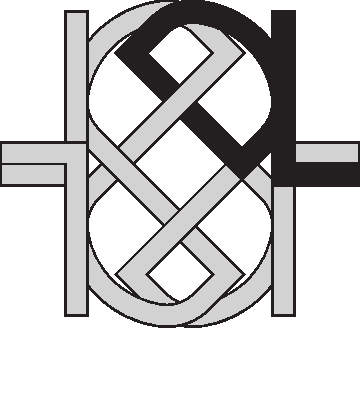
\includegraphics[align=c,height=1.25\baselineskip]{dl}\kern-1.5pt%
  \endgroup
}

%%
%% AMS Theorems
\usepackage{amsthm}
\newtheorem{theorem}{Theorem}
\newtheorem{definition}{Definition}
\newtheorem{example}{Example}

%%%%%%%%%%%%%%%%%%%%%%%%%%%%%%%%%%%%%%%%
%%% OUR SETTINGS
\usepackage[capitalise]{cleveref}
\usepackage{amsmath}
\usepackage{amssymb}
\usepackage{mathtools}
\usepackage{algorithm}
\usepackage{algpseudocode}
% \usepackage{theorem}
\usepackage{xspace}
\usepackage{dl}
\usepackage{url}
%\usepackage[numbers]{natbib}
\clubpenalty = 10000
\widowpenalty = 10000
\displaywidowpenalty = 10000
% theorems and the like
% \newtheorem{theorem}{Theorem}
\newtheorem{lemma}{Lemma}
% \newtheorem{proposition}{Proposition}
% \newtheorem{corollary}{Corollary}

% \theorembodyfont{\rmfamily}
% \newtheorem{definition}{Definition}
% \newtheorem{example}{Example}

% \theorembodyfont{\slshape}
% \newtheorem{assumption}{Assumption}

% \theorembodyfont{\slshape}
% \newtheorem{hypothesis}{Hypothesis}

% \newenvironment{justification}{\textsf{Justification:}}{\hfill $\Box$}
%\newenvironment{proof}{\noindent\textsc{proof:}}{\hfill $\square$ \bigskip}


\newcommand{\AL}{\ensuremath{\mathcal{AL}}\xspace}
\newcommand{\ALC}{\ensuremath{\mathcal{ALC}}\xspace}
\newcommand{\SROIQ}{\ensuremath{\mathcal{SROIQ}}\xspace}
\newcommand{\onto}[1]{\ensuremath{\mathsf{#1}}}
\usepackage[colorinlistoftodos]{todonotes}

\newcommand{\cg}
{\ensuremath{\blacktriangle}\xspace}
%{\ensuremath{\dot{\sqcup}}\xspace}

\newcommand{\todoT}[1]{\todo[fancyline,size=\small,color=orange!40]{\textbf{TBD:} #1}\xspace}
\newcommand{\todoR}[1]{\todo[fancyline,size=\small,color=orange!40]{\textbf{rc:} #1}\xspace}

\newcommand{\todoO}[1]{\todo[fancyline,size=\small,color=red!20]{\textbf{ok:} #1}\xspace}

\newcommand{\tododo}[1]{\todo[fancyline,size=\small,color=red!60]{\textbf{ToDO:} #1}\xspace}
\newcommand{\todoin}[1]{\todo[inline,size=\small,color=green!20]{\textbf{HERE:} #1}\xspace}


%\usepackage{pgf}https://preview.overleaf.com/public/pqghhhhwjqpw/images/986e3685291cb332a5fbe5a979b5045d2e649a43.jpeg
\usepackage{tikz}
%\usetikzlibrary{arrows,automata}
\usetikzlibrary{positioning,calc,backgrounds}

%%%%%%%MACROS%%%%%%%%
\newcommand{\Imc}{\ensuremath{\mathcal{I}}\xspace}
\newcommand{\Jmc}{\ensuremath{\mathcal{J}}\xspace}
\newcommand{\Tmc}{\ensuremath{\mathcal{T}}\xspace}
\newcommand{\Amc}{\ensuremath{\mathcal{A}}\xspace}
\newcommand{\Rmc}{\ensuremath{\mathcal{R}}\xspace}
\newcommand{\Omc}{\ensuremath{\mathcal{O}}\xspace}
\newcommand{\Omcref}{\ensuremath{\mathcal{O}_\mathrm{ref}}\xspace}
\newcommand{\Omcfull}{\ensuremath{\mathcal{O}_\mathrm{full}}\xspace}
\newcommand{\Ontology}{\Omc}

% \newcommand{\sub}{\ensuremath{\mathsf{sub}}\xspace}
\newcommand{\subr}{\ensuremath{\mathsf{subr}}\xspace}

\newcommand{\EL}{\ensuremath{\mathcal{E\!L}}\xspace}
\newcommand{\elpp}{\ensuremath{\mathcal{E\!L}^{++}}\xspace}
% \newcommand{\DL}{{\ensuremath{\mathcal{DL}}}\xspace}

\newcommand{\Inf}{{\ensuremath{\mathsf{Inf}}}\xspace}
\newcommand{\qual}{{\ensuremath{\mathsf{IIC}}}\xspace}

\newcommand{\Tup}{{\ensuremath{\mathsf{UpCover}_\Ontology}}\xspace}
\newcommand{\Tdown}{{\ensuremath{\mathsf{DownCover}_\Ontology}}\xspace}
\newcommand{\gammaT}{{\ensuremath{\gamma_\mathcal{T}}}\xspace}
\newcommand{\rhoT}{{\ensuremath{\rho_\mathcal{T}}}\xspace}
%\newcommand{\gammaT}{{\ensuremath{\gamma_{\mathcal{T}}}\xspace}
%\newcommand{\rhoT}{{\ensuremath{\rho_{\mathcal{T}}}\xspace}

\newcommand{\disjoint}{\ensuremath{\mathit{disjoint}}\xspace}
\newcommand{\self}{\ensuremath{\mathit{Self}}\xspace}
\newcommand{\less}[2]{\ensuremath{\leq #1~#2}\xspace}
\newcommand{\more}[2]{\ensuremath{\geq #1~#2}\xspace}
\newcommand{\nominal}[1]{\ensuremath{\{#1\}}\xspace}

\newcommand{\inv}{\ensuremath{\mathit{inv}}\xspace}
\newcommand{\refine}{\ensuremath{\mathop{\uparrow}}\xspace}
\newcommand{\corefine}{\ensuremath{\mathop{\downarrow}}\xspace}
%\DeclareMathOperator*{\argmax}{\mathsf{arg\,max}}
\DeclareMathOperator*{\argmax}{\mathsf{argmax}}

%%%%%%%%%%%%%%%%%%%%%%%%%%%%%%%%%%%%%%%%

%%
%% end of the preamble, start of the body of the document source.
\begin{document}

%%
%% Rights management information.
%% CC-BY is default license.
\copyrightyear{2023}
\copyrightclause{Copyright for this paper by its authors.
  Use permitted under Creative Commons License Attribution 4.0
  International (CC BY 4.0).}

%%
%% This command is for the conference information
\conference{\DLLogo{} DL 2023: 36th International Workshop on Description Logics,
  September 2--4, 2023, Rhodes, Greece}

%%
%% The "title" command
\title{Making Axiom Weakening Work in SROIQ}

%%
%% The "author" command and its associated commands are used to define
%% the authors and their affiliations.
\author[1]{Roland Bernard}[
email=roland.bernard@student.unibz.it,
]
\author[1]{Oliver Kutz}[
email=oliver.kutz@unibz.it,
]
\author[1]{Nicolas Troquard}[
email=nicolas.troquard@unibz.it,
]
\address[1]{
Free University of Bozen-Bolzano, Italy
}

%%
%% The abstract is a short summary of the work to be presented in the
%% article.
\begin{abstract}
Axiom weakening is a technique that allows for a fine-grained repair of inconsistent ontologies. Its main advantage is that it repairs ontologies by making axioms
less restrictive rather than by deleting them, employing refinement operators. In this paper, we build on previously introduced axiom weakening for \ALC, and show how it can be extended to deal with \SROIQ, the expressive and decidable description logic underlying OWL 2 DL. The main problem here is to ensure that the regularity conditions of \SROIQ are preserved in the weakening process, as not every weaker axiom can be inserted into an ontology without compromising regularity.
We present a basic regularity-preserving weakening approach for \SROIQ, describe briefly a prototype implementation realising it, and perform and discuss basic evaluations of the approach.
\end{abstract}

%%
%% Keywords. The author(s) should pick words that accurately describe
%% the work being presented. Separate the keywords with commas.
\begin{keywords}
  Description Logic \sep
  Knowledge Refinement \sep
  Axiom Weakening \sep
  Ontology Debugging \sep
  SROIQ \sep
  Prot\'eg\'e
\end{keywords}

%%
%% This command processes the author and affiliation and title
%% information and builds the first part of the formatted document.
\maketitle

\section{Introduction}

Many approaches to repairing inconsistent ontologies amount to identifying problematic axioms and then removing them (e.g., ~\cite{ScCo03,kalyanpur2005debugging,kalyanpur2006repairing,BaPS07}). Whilst this approach is obviously sufficient to guarantee that the obtained ontology is consistent, it tends to lead to information loss as a secondary effect, as we outlined in detail in previous work \cite{troquard2018repairing,confalonieri2020towards}, where also a more extensive discussion of related work can be consulted.   Further, this information loss can be reduced by weakening the inferential power of an axiom rather than by deleting it \cite{du2014practical,AMAI-2018,DBLP:conf/kr/BaaderKNP18,troquard2018repairing,confalonieri2020towards}. 
%
In \cite{troquard2018repairing}, axiom weakening using refinement operators has been described for \ALC and experimentally evaluated, showing that axiom weakening is able to retain more information than deletion. In \cite{confalonieri2020towards}, the axiom weakening has been extended to include many aspects of \SROIQ, notably omitting, however, the weakening of RBox axioms. The authors of \cite{confalonieri2020towards} further show that the proposed repair by iterated weakening almost surely terminates. 

In this  paper, we extend the previous work on axiom weakening in DLs by extending the underlying basic principles to the logic \SROIQ, including also the weakening of RIAs. We discuss a number of scenarios where weakening can impact regularity of \SROIQ Rboxes, and provide a framework where this is avoided. Additionally, by implementing the proposed refinement and weakening operators we are able to perform experimental evaluation, also on ontologies using the more expressive features of \SROIQ. The results reaffirm the results of \cite{troquard2018repairing} for the case of \SROIQ, namely that weakening may significantly outperform deletion.

\section{Axiom Weakening for \SROIQ}

\noindent
We first give a brief description of the DL \SROIQ; for full details, see \cite{HorrocksKutzSattlerKR2006,Kazakov08,baader_horrocks_lutz_sattler_2017}. 

\subsection{Defining \SROIQ}

% describe the SROIQ syntax
% describe roles and concepts
The syntax of \SROIQ is based on a vocabulary of three disjoint sets $N_C$, $N_R$, $N_I$ of, respectively, \emph{concept names}, \emph{role names}, and \emph{individual names}. The sets of, respectively, \SROIQ  \emph{roles} and \SROIQ \emph{concepts} are generated by the following grammar.
{\footnotesize
\begin{alignat*}{2}
  R, S &::={} && U \mid r \mid r^{-} \enspace,\\
  C &::= && \bot \mid \top \mid A \mid \neg C \mid C \sqcap C \mid C \sqcup C \mid \forall R.C \mid \exists R.C \mid \\ 
  &&& \more n S.C \mid \less n S.C \mid \exists S.\self \mid \nominal i \enspace,
\end{alignat*}
}
\noindent where $A \in N_C$ is a concept name, $r \in N_R$ is a role name, $i \in N_I$ is an individual name and $n \in \mathbb{N}_0$ is a non-negative integer. 
%
$U$ is the universal role. $S$ is a \emph{simple role} in the RBox $\Rmc$ (see below). In the following, $\Lmc(N_C, N_R, N_I)$ and $\Lmc(N_R) = N_R \cup \{U\} \cup \{r^- \mid r \in N_R\}$ denote, respectively, the set of concepts and roles that can be built over $N_C$, $N_R$, and $N_I$ in \SROIQ.

We next define the notions of TBox, ABox, and (regular) RBox, of complex role inclusions, and of (non-)simple roles:
% describe the TBox, ABox and RBox statements
A \emph{TBox} $\Tmc$ is a finite set of concept inclusions (GCIs) of the form $C \sqsubseteq D$ where $C$ and $D$ are concepts. The TBox is used to store terminological knowledge concerning the relationship between concepts. 
%
An \emph{ABox} $\Amc$ is a finite set of statements of the form $C(a)$, $R(a,b)$, $\lnot R (a,b)$, $a = b$, and $a \not= b$, where $C$ is a concept, $R$ is a role and $a$ and $b$ are individual names. The ABox expresses knowledge regarding individuals in the domain. 
%
An \emph{RBox} $\Rmc$ is a finite set of role inclusions (RIAs) of the form $R_1 \circ \cdots \circ R_n \sqsubseteq R$, and disjoint role axioms $\disjoint(S_1, S_2)$ where $R$, $R_1$, $\dots$, $R_n$, $S_1$, and $S_2$ are roles. $S_1$ and $S_2$ are simple (defined next) in the RBox $\Rmc$. The special case of $n = 1$ is a simple role inclusion, while we call the cases where $n > 1$ \emph{complex role inclusions}. The RBox represents knowledge about the relationships between roles.

% describe simple and complex roles since it is relevant
The set of \emph{non-simple} roles in $\Rmc$ is the smallest set such that: $U$ is non-simple; any role $R$ that appears as the super role of a complex RIA $R_1 \circ \cdots \circ R_n \sqsubseteq R$ where $n > 1$ is non-simple; any role $R$ that appears on the right-hand side of a simple RIA $S \sqsubseteq R$ where $S$ is non-simple, is also non-simple; and a role $r$ is non-simple if and only if $r^-$ is non-simple.
All other roles are \emph{simple}.

% describe regularity since it is relevant
For convenience, let us define the function $\inv(R)$ such that $\inv(r) = r^-$ and $\inv(r^-) = r$ for all role names $r \in N_R$. 
%
An RBox $\Rmc$ is  \emph{regular} if there exists a preorder $\preceq$, i.e., a transitive and reflexive relation, over the set of roles appearing in $\Rmc$, such that $R \preceq S \iff \inv(R) \preceq S$ and all RIAs are of the forms:
$\inv(R) \sqsubseteq R$,
$R \circ R \sqsubseteq R$,
$S \sqsubseteq R$, $R \circ S_1 \circ \cdots \circ S_n \sqsubseteq R$,
$S_1 \circ \cdots \circ S_n \circ R \sqsubseteq R$, or
$S_1 \circ \cdots \circ S_n \sqsubseteq R$,
where $n > 1$ and $R$, $S$, $S_1, \cdots, S_n$ are roles such that $S \preceq R$, $S_i \preceq R$, and $R \not\preceq S_i$ for $i = 1, \dots, n$. This regularity restriction has been chosen to align with the implementation of the OWL 2 DL \cite{motik2012ontology} profile checker in the OWL API \cite{horridge2011owl}. 

\begin{definition}
A \SROIQ  ontology $\Omc = \Tmc \cup \Amc \cup \Rmc$ consists of a TBox $\Tmc$, an ABox $\Amc$, and a RBox $\Rmc$ in the language of \SROIQ, and where the RBox $\Rmc$ is regular.
\end{definition}

% describe the semantics
% whats a interpretation, when is it a model
The semantics of \SROIQ is  defined using \emph{interpretations} $I = \langle \Delta^I, \cdot^I \rangle$, where $\Delta^I$ is a non-empty \emph{domain} and $\cdot^I$ is a function associating to each individual name $a$ an element of the domain $a^I \in \Delta^I$, to each concept $C$ a subset of the domain $C^I \subseteq \Delta^I$, and to each role $R$ a binary relation on the domain $R^I \subseteq \Delta^I \times \Delta^I$; see \cite{baader_horrocks_lutz_sattler_2017,HorrocksKutzSattlerKR2006} for further details. An interpretation $I$ is a \emph{model} for $\Omc$ if it satisfies all the axioms in $\Omc$.

% describe subsumptions of concepts and roles
Given two concepts $C$ and $D$ we say that $C$ is \emph{subsumed} by $D$ (or $D$ \emph{subsumes} $C$) with respect to the ontology $\Omc$, written $C \sqsubseteq_\Omc D$, if $C^I \subseteq D^I$ in every model $I$ of $\Omc$. Further, $C$ is \emph{strictly subsumed by} $D$, written $C \sqsubset_\Omc D$, if $C \sqsubseteq_\Omc D$ but not $D \sqsubseteq_\Omc C$. Analogously, given two roles $R$ and $S$, $R$ is subsumed by $S$ with respect to $\Omc$ ($R \sqsubseteq_\Omc S$) if $R^I \sqsubseteq S^I$ in all models $I$ of $\Omc$. Again, $R \sqsubset_\Omc S$ holds if $R \sqsubseteq_\Omc S$ but not $D \sqsubseteq_\Omc C$.

\subsection{Weakening, reference ontologies, covers, refinement operator}

\paragraph{The case of \ALC.}
Axiom weakening, as discussed in \cite{troquard2018repairing}, is based on refinement operators. Two types of refinement operators are used, a specialization operator and a generalization operator. They return for a given concept a set of, respectively, more specific or more general concepts. In \cite{troquard2018repairing} the proposed refinement operator is based on upward and downward cover sets. The upward or downward cover for a concept is the set of, respectively, the most specific generalization or most general specializations from the set of subconcepts.
%
Given an inconsistent ontology $\Omc = \Tmc \cup \Amc \cup \Rmc$, to be able to compute a non-trivial upcover and downcover, we first need to find a consistent subontology $O^\text{ref}$ of $\Omc$ to serve as \emph{reference ontology}. One approach is to pick a random maximally consistent subset of $\Omc$ and choose it as reference ontology $O^\text{ref}$; another is to choose the intersection of all maximally consistent subsets of $\Ontology$ (e.g.,~\cite{LLRRS10}).

Once a reference ontology $O^\text{ref}$ has been chosen, and as long as $\Omc$ is inconsistent, we select a ``bad axiom'' and replace it with a random weakening of it with respect to $O^\text{ref}$.
%
We can randomly sample a number of (or all the) minimally inconsistent subsets of axioms $I_1, I_2, \ldots I_k \subseteq \Omc$ and return one axiom in $\Tmc \cup \Amc$ from the ones occurring the most often.
%
Weakening of GCIs is performed by either using the specialization operator to refine the left-hand side or the generalization operator for the right-hand side. For class assertions, the concept is refined using the generalization operator.

% explain the complications of weakening SROIQ
\paragraph{The case of \SROIQ.}
The main difficulties that arise when weakening axioms in \SROIQ ontologies, and especially when weakening RIAs, are related to ensuring that the constraints on the use of non-simple roles and the regularity of the RBox as a whole are maintained. Not every weaker axiom can be inserted into a valid \SROIQ ontology without causing a violation of these restrictions, as shown in the next example.

% example of the complications of weakening SROIQ
\begin{example}
  Take the ontology $\Omc = \{ r \circ s \circ r \sqsubseteq t, r \sqsubseteq s, \top \sqsubseteq \forall t.\bot, \exists s.\self \sqsubseteq \top \}$. Since $t$ is empty in every model of this ontology, the axiom $r \sqsubseteq s$ could be weakened to $t \sqsubseteq s$ if we ignore the additional constraints. This would result in an ontology where $s$ is non-simple, which is not allowed since $s$ is used as part of a self constraint.
  Additionally, using this weakening would also cause a non-regular RBox, because for any preorder $\preceq$, $t \not\preceq s$ must hold for the complex RIA and $t \preceq s$ must hold for the new axiom. Yet, this is a contradiction.
\end{example}

% lay out the constraints that we want to maintain
To prevent these kinds of issues, we restrict how concepts are refined and RIAs weakened. In \cite{confalonieri2020towards}, the refinement of RIAs was not considered at all to avoid these problems. In this paper, however, we have extended the axiom weakening operator to handle also RIAs. To achieve this, we must ensure that only simple roles are used when weakening disjoint role axioms or refining cardinality and $\self$ constraints.  
%
Further, it must be guaranteed that all roles that are currently used in such contexts remain simple when adding the weakened axioms to the ontology. Finally, the addition of a weakened axiom must maintain the regularity of the RBox. 

\medskip\noindent
We now discuss which restrictions we applied in order to satisfy these requirements.

\subsection{Saving Regularity}

% explain how each of them can be ensured
Firstly, the covers and refinement operators for roles operate only on roles that are simple. A similar restriction has already been applied in the refinement operator suggested in \cite{confalonieri2020towards}. Restricting the refinement to simple roles guarantees that the new axioms created by weakening will not contain non-simple roles in axioms or concepts where they are not allowed. An important detail that was not considered in \cite{confalonieri2020towards} is that the roles over which the covers operate must be simple in all ontologies that the weaker axioms are used in. It is therefore not generally sufficient to use the roles that are simple in the reference ontology, since the reference ontology may not contain all RBox axioms, and therefore contain simple roles that are not simple in the full ontology. For this reason, we give to the upward and downward cover as an argument not only the reference ontology $\Omcref$, but also the full ontology $\Omcfull$. Both $\Omcref$ and $\Omcfull$ share the same vocabulary $N_I$, $N_C$, and $N_R$. We assume that $\Omcref \subseteq \Omcfull$. In the context of repairing inconsistent ontologies, $\Omcfull$ can be chosen to be the inconsistent ontology that we want to repair.

Then, to ensure further that by adding weakened axioms we do not cause a constraint violation in existing axioms and concepts, we choose the allowed weakening for RIAs such that all roles that are simple in $\Omcfull$, are also simple after adding to it a weakening of one of its axioms. We observe that for complex RIAs $S_1 \circ \cdots \circ S_n \sqsubseteq R$ we should not refine the role $R$. Since all roles returned by our refinement operator are simple in $\Omcfull$,  a replacement of $R$ with a refinement $R'$ would create an axiom which would make a role which was simple in $\Omcfull$ now non-simple. A similar argument can be made for refining $R$ in a simple RIA $S \sqsubseteq R$ where the role $S$ is non-simple in $\Omcfull$. So the only way to refine the super role during the weakening of a RIA is when it is a simple RIA and additionally the sub role of the axiom is simple in $\Omcfull$.

When it comes to refining the left-hand side of RIAs, we do not need any special restrictions. The main significant observation is that all roles that are returned by the refinement will be simple. This means that in a simple RIA $R \sqsubseteq S$, even if $S$ is simple, replacing $R$ with another simple role will not cause $S$ to become non-simple. For a complex RIA $S_1 \circ \cdots \circ S_n \sqsubseteq R$ on the other hand, the role $R$ must already have been non-simple in $\Omcfull$, and replacing any $S_i$ with a refinement has no effect on which roles are simple.

A more interesting question is whether such a weakening may still cause a non-regular RBox. The important insight is that simple roles are always allowed on the left-hand side of a RIA. While this is more directly evident in some alternative definitions of regularity (e.g., \cite{rudolph2011foundations}) it is not so apparent from the one presented in this paper.
%
Intuitively, the constraints given above for regularity disallow dependency cycles that contain complex RIAs. Simple roles cannot be part of such a cycle, since the cycle must contain at least one complex RIA to be a violation of the constraint, and all roles that depend in this sense on a complex RIA must be non-simple. 
%
A more formal justification for this fact is given in the \hyperref[proof:regularity]{proof} for \Cref{lem:regularity}.
Since all refinements of the left-hand side of RIAs are performed using simple roles, these cannot lead to a non-regular RBox. Further, refinements of the super role of RIAs are only performed on simple RIAs $S \sqsubseteq R$ where $S$ is a simple role. Since $S$ is simple in this case, all refinements of $R$ are allowed, potentially also if the refinement yielded a non-simple role.

\begin{definition}
  Let $\Omc$ be a \SROIQ ontology. The set of \emph{subconcepts} of $\Omc$ is given by 
  {\footnotesize
  \begin{align*}
    \sub(\Omc) = \{\top, \bot\} \cup \bigcup_{C(a) \in \Omc} \sub(C) \cup \bigcup_{C \sqsubseteq D \in \Omc} ( \sub(C) \cup \sub(D) ) \enspace,
  \end{align*}
  }
  where $\sub(C)$ is the set of \emph{subconcepts} in $C$.
\end{definition}

% define upward and downward covers
We will define now the upward and downward cover sets for concepts and roles. Intuitively, for a given concept the upward cover is the set of the most specific generalizations from the (fixed) set of subconcepts or roles, while the downward cover set contains the most general specializations from the same set of subconcepts and roles. (Note that the related open search for e.g.\ a least common subsumer is in general a harder problem \cite{baader2003least}.) We define the upward and downward cover additionally also for non-negative integers, as they will be useful in the refinement of cardinality constraints.

\begin{definition} \label{def:covers}
  Let $\Omcfull$ and $\Omcref \subseteq \Omcfull$ be two \SROIQ ontologies that share the same vocabulary $N_C$, $N_R$, and $N_I$. The \emph{upward cover} and \emph{downward cover} for a concept $C$ are given by
  {\footnotesize
  \begin{alignat*}{2}
    \UpC_{\Omcref,\Omcfull}(C) &= \{ &&D \in \sub(\Omcfull) \mid C \sqsubseteq_\Omcref D \text{ and } \\
    &&&\nexists D' \in \sub(\Omcfull) \text{ with } C \sqsubset_\Omcref D' \sqsubset_\Omcref D \} \enspace, \\
    \DownC_{\Omcref,\Omcfull}(C) &= \{ &&D \in \sub(\Omcfull) \mid D \sqsubseteq_\Omcref C \text{ and } \\
    &&&\nexists D' \in \sub(\Omcfull) \text{ with } D \sqsubset_\Omcref D' \sqsubset_\Omcref C \} \enspace.
  \end{alignat*}
  }
  The upward and downward covers for a role $R$ are given by
  {\footnotesize
  \begin{alignat*}{2}
    \UpC_{\Omcref,\Omcfull}(R) &= \{ &&S \in \Lmc(N_R) \mid R \sqsubseteq_\Omcref S \text{ and } \\
    &&& \nexists S' \in \Lmc(N_R) \text{ with } R \sqsubset_\Omcref S' \sqsubset_\Omcref S \text{ and } \\
    &&& S, S' \text{ are simple in } \Omcfull \} \enspace, \\
    \DownC_{\Omcref,\Omcfull}(R) &= \{ &&S \in \Lmc(N_R) \mid S \sqsubseteq_\Omcref R \text{ and } \\
    &&&\nexists S' \in \Lmc(N_R) \text{ with } S \sqsubset_\Omcref S' \sqsubset_\Omcref R \text{ and } \\
    &&& S, S' \text{ are simple in } \Omcfull \} \enspace.
  \end{alignat*}
  }
  The upward and downward covers for a non-negative integer $n$ are given by
  {\footnotesize
  \begin{alignat*}{2}
    \UpC_{\Omcref,\Omcfull}(n) &= \{ n, n + 1 \} \enspace, \\
    \DownC_{\Omcref,\Omcfull}(R) &=
    \begin{cases*}
      \{ n \} & \text{ if } n = 0 \\
      \{ n, n - 1 \} & \text{ if } n > 0
    \end{cases*} \enspace.
  \end{alignat*}
  }
\end{definition}

Since they operate only over the subconcepts of $\Omcfull$, on their own, the upward and downward covers of concepts are missing some interesting refinements.
\begin{example} \label{exa:up-cover}
  Let $N_C = \{A, B, C\}$, $N_R = \{ r, s \}$, and $\Omc = \{A \sqsubseteq B, r \sqsubseteq s\}$. $\sub(\Omc) = \{\top, \bot, A, B\}$. The upward cover of $C \sqcup A$ is equal to $\UpC_{\Omc,\Omc}(C \sqcup A) = \{ \top \}$. The potentiality refinement to $C \sqcup B$ will be missed even by iterated application of the upward cover because $C \sqcup B \not\in \sub(\Omc)$. Similarly, $\UpC_{\Omc,\Omc}(\forall r.A) = \{ \top \}$, even if \  $\forall r.B$ and $\forall s.A$ are reasonable generalizations.
\end{example}

% define the abstract refinement operator
% define the concrete generalization and specialization operator
To also capture these omissions, we define generalization and specialization operators that exploit the recursive structure of the concept being refined to generate more complex refinements. For convenience, we also define these operators for roles.

\begin{definition}
  Let $\refine$ and $\corefine$ be two functions with domain $\Lmc(N_C, N_R, N_I) \cup \Lmc(N_C) \cup \mathbb{N}_0$. They map every concept to a finite subset of $\Lmc(N_C, N_R, N_I)$, every role to a subset of $\Lmc(N_C)$, and every non-negative integer to a finite subset of $\mathbb{N}_0$.
  The \emph{abstract refinement operator} is defined recursively by induction on the structure of concepts as follows.
  {\footnotesize
  \begin{alignat*}{2}
    \zeta_{\refine,\corefine}(A) &= &&\refine(A) \quad, A \in N_C \cup \{\top, \bot\} \enspace, \\
    \zeta_{\refine,\corefine}(\lnot C) &= &&\refine(\lnot C) \cup \{ \lnot C' \mid C' \in \zeta_{\corefine,\refine}(C) \} \enspace, \\
    \zeta_{\refine,\corefine}(C \sqcap D) &= &&\refine(C \sqcap D) \cup \{ C' \sqcap D \mid C' \in \zeta_{\refine,\corefine}(C) \}
    \cup \{ C \sqcap D' \mid D' \in \zeta_{\refine,\corefine}(D) \} \enspace, \\
    \zeta_{\refine,\corefine}(C \sqcup D) &= &&\refine(C \sqcup D) \cup \{ C' \sqcup D \mid C' \in \zeta_{\refine,\corefine}(C) \}
    \cup \{ C \sqcup D' \mid D' \in \zeta_{\refine,\corefine}(D) \} \enspace, \\
    \zeta_{\refine,\corefine}(\forall R.C) &= &&\refine(\forall R.C) \cup \{ \forall R'.C \mid R' \in \corefine(R) \}
    \cup \{ \forall R.C' \mid C' \in \zeta_{\refine,\corefine}(C) \} \enspace, \\
    \zeta_{\refine,\corefine}(\exists R.C) &= &&\refine(\exists R.C) \cup \{ \exists R'.C \mid R' \in \refine(R) \}
    \cup \{ \exists R.C' \mid C' \in \zeta_{\refine,\corefine}(C) \} \enspace, \\
    &&& \text{\SROIQ concepts:} \\
    \zeta_{\refine,\corefine}(\nominal i) &= &&\refine(\nominal i) \enspace, \\
    \zeta_{\refine,\corefine}(\exists R.\self) &= &&\refine(\exists R.\self) \cup \{ \exists R'.\self \mid R' \in \refine(R) \} \enspace, \\
    \zeta_{\refine,\corefine}(\more n R.C) &= &&\refine(\more n R.C) \cup \{ \more n R'.C \mid R' \in \refine(R) \} \\
    &&& \cup \{ \more n R.C' \mid C' \in \zeta_{\refine,\corefine}(C) \}
    \cup \{ \more n' R.C \mid n' \in \corefine(n) \} \enspace, \\
    \zeta_{\refine,\corefine}(\less n R.C) &= &&\refine(\less n R.C) \cup \{ \less n R'.C \mid R' \in \corefine(R) \} \\
    &&& \cup \{ \less n R.C' \mid C' \in \zeta_{\corefine,\refine}(C) \}
    \cup \{ \less n' R.C \mid n' \in \refine(n) \} \enspace, \\
    &&& \text{\SROIQ roles:} \\
    \zeta_{\refine,\corefine}(R) &= &&\refine(R) \enspace.
  \end{alignat*}
  }
  From the abstract refinement operator $\zeta_{\refine,\corefine}$, two concrete refinement operators, the \emph{generalization operator} and \emph{specialization operator} are, respectively, defined as
  {\footnotesize
  \begin{align*}
    \gamma_{\Omcref,\Omcfull} &= \zeta_{\UpC_{\Omcref,\Omcfull},\DownC_{\Omcref,\Omcfull}} \enspace \text{and} \\
    \rho_{\Omcref,\Omcfull} &= \zeta_{\DownC_{\Omcref,\Omcfull},\UpC_{\Omcref,\Omcfull}} \enspace.
  \end{align*}
  }
\end{definition}

Revisiting the case in \Cref{exa:up-cover} we observe that $\gamma_{\Omc,\Omc}(C \sqcup A) = \{ \top, \top \sqcup A, C \sqcup A, C \sqcup B \}$ does contain $C \sqcup B$ as a possible refinement. Similarly, $\gamma_{\Omc,\Omc}(\forall r.A) = \{ \top, \forall r.A, \forall s.A, \forall r.B \}$ contains $\forall r.B$. We will show now some basic properties of $\gamma_{\Omcref,\Omcfull}$ and $\rho_{\Omcref,\Omcfull}$ that will prove useful in the remainder of this paper.

\begin{lemma}\label{lem:basic}
  For every pair of \SROIQ ontologies $\Omcref, \Omcfull$ and every pair of concepts or roles $X, Y \in \Lmc(N_C, N_R, N_I) \cup \Lmc(N_R)$:
  \newcommand\litem[1]{\item{\bfseries #1:\enspace }}
  \begin{enumerate}
    \litem{generalisation}\label{lem:generalisation} if $X \in \gamma_{\Omcref,\Omcfull}(Y)$ then $Y \sqsubseteq_{\Omcref} X$ \\
    \textbf{specialisation:\enspace} if $X \in \rho_{\Omcref,\Omcfull}(Y)$ then $X \sqsubseteq_{\Omcref} Y$
    \litem{generalisation finiteness} $\gamma_{\Omcref,\Omcfull}(X)$ is finite \\
    \textbf{specialisation finiteness:\enspace} $\rho_{\Omcref,\Omcfull}(X)$ is finite
  \end{enumerate}
\end{lemma}

% define the weakening operator
We define now the \emph{axiom weakening operator} using these generalization and specialization operators.

\begin{definition}
  Given an axiom $\phi$, the set of \emph{weakenings} with respect to the reference ontology $\Omcref$ and full ontology $\Omcfull$, written $g_{\Omcref,\Omcfull}(\phi)$ is defined such that
  {\footnotesize
  \begin{alignat*}{2}
    g_{\Omcref,\Omcfull}(C \sqsubseteq D) &={} &&\{ C' \sqsubseteq D \mid C' \in \rho_{\Omcref,\Omcfull} (C) \} \cup \{ C \sqsubseteq D' \mid D' \in \gamma_{\Omcref,\Omcfull}(D) \} \enspace, \\
    g_{\Omcref,\Omcfull}(C(a)) &={} && \{ C'(a) \mid C' \in \gamma_{\Omcref,\Omcfull}(C) \} \enspace, \\
    g_{\Omcref,\Omcfull}(R(a, b)) &={} && \{ R'(a, b) \mid R' \in \gamma_{\Omcref,\Omcfull}(R) \} \cup \{ R(a, b), \bot \sqsubseteq \top \} \enspace, \\
    g_{\Omcref,\Omcfull}(\lnot R(a, b)) &={} && \{ \lnot R'(a, b) \mid R' \in \rho_{\Omcref,\Omcfull}(R) \} \cup \{ \lnot R(a, b), \bot \sqsubseteq \top \} \enspace, \\
    g_{\Omcref,\Omcfull}(a = b) &={} && \{ a = b, \bot \sqsubseteq \top \} \enspace,
    \quad g_{\Omcref,\Omcfull}(a \not= b) = \{ a \not= b, \bot \sqsubseteq \top \} \enspace, \\
    g_{\Omcref,\Omcfull}(\disjoint(R, S)) &={} &&\{ \disjoint(R', S) \mid R' \in \rho_{\Omcref,\Omcfull} (R) \} \\
    &&& \cup \{ \disjoint(R, S') \mid S' \in \rho_{\Omcref,\Omcfull}(S) \} \\
    &&& \cup \{ \disjoint (R, S), \bot \sqsubseteq \top \} \enspace, \\
    g_{\Omcref,\Omcfull}(S_1 \circ \cdots \circ S_n \sqsubseteq R) &={} && \{ S_1 \circ \cdots \circ S_i' \circ \cdots \circ S_n \sqsubseteq R \mid S_i' \in \rho_{\Omcref,\Omcfull}(S_i) \text{ for } i = 1, \dots, n \} \\
    &&& \cup \{ S_1 \sqsubseteq R' \mid R' \in \gamma_{\Omcref,\Omcfull} \text{ and } n = 1 \text{ and } S_1 \text{ is simple in } \Omcfull \} \\
    &&& \cup \{ S_1 \circ \cdots \circ S_n \sqsubseteq R, \bot \sqsubseteq \top \} \enspace.
  \end{alignat*}
  }
\end{definition}

The axioms in the set $g_{\Omcref,\Omcfull}(\phi)$ are indeed weaker than $\phi$ for every axiom $\phi$, in the sense that, given the reference ontology $\Omcref$, $\phi$ entails them and the opposite in not necessarily true.

\begin{lemma} \label{lem:weaker}
  For every \SROIQ axiom $\phi$, if $\phi' \in g_{\Omcref,\Omcfull}(\phi)$, then $\phi \models_\Omcref \phi'$
\end{lemma}

Clearly, replacing an axiom in the full ontology with a weakening cannot reduce the number of models of the ontology. However, for the weakening to be useful in practice, we must show additionally that by adding the weakened axioms to the ontology will not violate any of the constraints that ensure the decidability of \SROIQ. To do this, we show first that all roles that are simple in $\Omcfull$ are also simple in the ontology obtained by adding the weakening of any axiom.

% proof that the constrains are retained
\begin{lemma} \label{lem:simple-roles}
  Let $\Omc$ be an ontology such that all simple roles of $\Omcfull$ are also simple in $\Omc$. For every axiom $\phi \in \Omc$ and role $R$, if $\phi' \in g_{\Omcref,\Omcfull}(\phi)$ and $R$ simple in $\Omc$, then $R$ is simple in $\Omc \cup \{ \phi' \}$.
\end{lemma}

Note that removal of axioms will never cause a role that was previously simple to become non-simple, so all roles simple in $\Omc$ are also simple in $\Omc \setminus \{ \phi \} \cup\{ \phi' \}$. Further, it should be noted that repeated replacement of axioms with weakened axioms keeps simple roles simple. This is an important observation, since repeated weakening is required for the proposed ontology repair algorithm.

\begin{lemma} \label{lem:regularity}
  Let $\Omc$ be an ontology such that all simple roles of $\Omcfull$ are also simple in $\Omc$. For every axiom $\phi \in \Omc$, if $\phi' \in g_{\Omcref,\Omcfull}(\phi)$ and the RBox of $\Omc$ is regular, then the RBox of $\Omc \cup \{ \phi' \}$ is also regular.
\end{lemma}

Like for the invariant on simple roles, also regularity is maintained by repeated replacement of axioms with weakenings. With the help of \Cref{lem:simple-roles} and \Cref{lem:regularity} we can now sketch a proof showing that adding weakened axioms to a \SROIQ ontology will yield another valid \SROIQ ontology.

\begin{theorem} \label{lem:global-constraints}
  Given that $\Omcref$ and $\Omcfull$ are valid \SROIQ ontologies. For every axiom $\phi \in \Omcfull$, if $\phi' \in g_{\Omcref,\Omcfull}(\phi)$, then $\Omcfull \cup \{ \phi' \}$ is a valid \SROIQ ontology.
\end{theorem}

\section{Implementing and Evaluating Axiom Weakening for \SROIQ}

% explain how the weakening is used for repair
The refinement operators and axiom weakening have previously been implemented for \ALC in \cite{troquard2018repairing}. Based on this, we have extended the implementation to cover the full range of \SROIQ axioms and concepts.\footnote{The source code for the implementation is available at \url{https://github.com/rolandbernard/ontologyutils}.} The concept refinement and axiom weakening operators for \SROIQ have been implemented as discussed above. Further, we implemented a repair algorithm using the axiom weakening operator based on the procedures already proposed in \cite{troquard2018repairing} and \cite{confalonieri2020towards}. The implementation performs weakening in OWL 2 DL \cite{motik2012ontology} and is implemented in Java using the OWL API \cite{horridge2011owl}. A plug-in for the ontology development tool Protégé has also been implemented, but will not be discussed in detail in this paper.\footnote{The Protégé plugin is available at \url{https://github.com/rolandbernard/protege-weakening}.} The plug-in allows for manually weakening axioms and executing the automatic repair algorithm.

\noindent
\begin{minipage}[t]{.5\textwidth}
  \begin{algorithm}[H]
    \footnotesize
    \begin{algorithmic}
      \State $\Omcfull \gets \Omc$
      \State $\Omcref \gets \textnormal{FindMaximalConsistentSubset(\Omc)}$
      \While{$\Omc$ is inconsistent}
        \State $\phi_\textnormal{bad} \gets \textnormal{FindBadAxiom}(\Omc)$
        \State $\Phi_\textnormal{weaker} \gets g_{\Omcref,\Omcfull}(\phi_\textnormal{bad})$
        \State $\phi_\textnormal{weaker} \gets \textnormal{SelectWeakerAxiom}(\Phi_\textnormal{weaker})$
        \State $\Ontology \gets (\Ontology \setminus \{\phi_\textnormal{bad}\}) \cup \{\phi_\textnormal{weaker}\}$
      \EndWhile
      \State Return $\Omc$
    \end{algorithmic}
    \caption{RepairOntologyWeaken($\Omc$)}
    \label{algo:repair-weaken}
  \end{algorithm}
\end{minipage}
\hfill
\begin{minipage}[t]{.45\textwidth}
  \begin{algorithm}[H]
    \footnotesize
    \begin{algorithmic}
      \While{$\Omc$ is inconsistent}
        \State $\phi_\textnormal{bad} \gets \textnormal{FindBadAxiom}(\Omc)$
        \State $\Ontology \gets \Ontology \setminus \{\phi_\textnormal{bad}\}$
      \EndWhile
      \State Return $\Omc$
    \end{algorithmic}
    \caption{RepairOntologyRemove($\Omc$)}
    \label{algo:repair-remove}
  \end{algorithm}
\end{minipage}
\vskip 8mm

% explain how the reference ontology is selected
% explain how bad axioms are selected
The automatic repair by weakening is implemented as shown in \Cref{algo:repair-weaken}. The reference ontology is selected by choosing a maximal consistent subset of the inconsistent ontology. In our implementation used for the evaluation in this paper, the reference ontology was selected by randomly sampling a maximal consistent subset. The procedure $\textnormal{FindBadAxiom}(\Omc)$ may be implemented in a number of ways. Here we consider an implementation that samples some (or all) of the minimal inconsistent subsets of $\Omc$ and selects as the bad axiom the one occurring most frequently. Then, $\textnormal{SelectWeakerAxiom}(\Phi_\textnormal{weaker})$ has been chosen such that is selects an axiom uniformly at random from $\Phi_\textnormal{weaker}$. For all experiments presented in this paper, the FaCT++ reasoner \cite{tsarkov2006fact++} was used to compute all entailment and consistency checks.

% explain how different repairs are compared
To experimentally evaluate the proposed axiom weakening operator in the context of its use in automatic repair of ontologies, we need some way to compare the quality of repair. As has already been discussed in \cite{troquard2018repairing}, the problem of deciding which of two possible repaired ontologies $\Omc_1$ or $\Omc_2$ is preferable is not generally well-defined. Similar to what has been proposed in \cite{troquard2018repairing} we will base the evaluation of the repairs on the size of the \emph{inferred class hierarchy}. To compare two possible repairs, we use the \emph{inferable information content} (IIC) as defined in \cite{troquard2018repairing}. The IIC  of an ontology $\Omc_1$ with respect to a second ontology $\Omc_2$, written $\qual(\Omc_1, \Omc_2)$, is a number between $0$ and $1$. Value closer to $0$ indicates that $\Omc_1$ contains more ``information'' than $\Omc_2$, while a value towards $1$ indicates the opposite. Some weaknesses of this measure when it comes to evaluating repairs, like the fact that only atomic concepts are considered, have already been discussed in \cite{troquard2018repairing}. For the case of repairing \SROIQ ontologies this is even more relevant, since the role hierarchy is entirely ignored.

\begin{definition}
  The \emph{inferred class hierarchy} of an ontology $\Omc$ is given by
  {\footnotesize
  \begin{align*}
    \Inf(\Omc) = \{ A \sqsubseteq B \mid A, B \in N_C \text{ and } \Omc \models A \sqsubseteq B \} \enspace.
  \end{align*}
  }

  The \emph{inferable information content} of an ontology $\Omc_1$ with respect to another ontology $\Omc_2$ is given by
  {\footnotesize
  \begin{align*}
    \qual(\Omc_1, \Omc_2) = \frac{\mathbf{card}(\Inf(\Omc_1) \setminus \Inf(\Omc_2))}{\mathbf{card}(\Inf(\Omc_1) \setminus \Inf(\Omc_2)) + \mathbf{card}(\Inf(\Omc_2) \setminus \Inf(\Omc_1))} \enspace,
  \end{align*}
  }
  where $\mathbf{card}(X)$ is the cardinality of the set $X$.
\end{definition}

% explain which ontologies where chosen and from where (BioPortal)
For the experimental evaluation we have selected ontologies of varying size and expressivity from BioPortal\footnote{\url{https://bioportal.bioontology.org/}} \cite{whetzel2011bioportal}. Additionally, the pizza ontology\footnote{Available from Protégé at \url{https://protege.stanford.edu/ontologies/pizza/pizza.owl}.} was included in the testing. Some characteristics of the used ontologies are shown in \Cref{table:ontologies}. On average, they contain about 289 axioms, 73 concept names, 29 role names, and 168 subconcepts.

\begin{table}
  \centering
  \scriptsize
  \begin{tabular}{|lllrrrr|}
    \hline
    Abbreviation & Name & Expressivity & Axioms & Concepts & Roles & Subconcepts \\
    \hline
    admin & Nurse Administrator & $\mathcal{ALCHOIF}$ & 229 & 42 & 29 & 144 \\
    ahso & Animal Health Surveillance Ontology & $\mathcal{ALCRIF}$ & 166 & 38 & 31 & 104 \\
    cdao & Comparative Data Analysis Ontology & $\mathcal{ALCROIQ}$ & 437 & 132 & 68 & 375 \\
    cdpeo & Chronic Disease Patient Education & $\mathcal{ALCHF}$ & 422 & 41 & 31 & 170 \\
    covid19-ibo & Covid19 Impact on Banking Ontology & $\mathcal{ALCH}$ & 288 & 160 & 33 & 227 \\
    ecp & Electronic Care Plan & $\mathcal{ALCRQ}$ & 127 & 33 & 17 & 99 \\
    emo & Enzyme Mechanism Ontology & $\mathcal{ALCHQ}$ & 368 & 157 & 24 & 255 \\
    evi & Evidence Graph Ontology & $\mathcal{ALCRI}$ & 143 & 30 & 38 & 69 \\
    falls & Falls Prevention & $\mathcal{ALCH}$ & 79 & 30 & 20 & 35 \\
    fo & Fern Ontology & $\mathcal{ALCHI}$ & 59 & 31 & 4 & 46 \\
    gbm & Glioblastoma & $\mathcal{ALCIF}$ & 603 & 108 & 28 & 227 \\
    gfvo & Genomic Feature and Variation Ontology & $\mathcal{ALCH}$ & 332 & 102 & 30 & 170 \\
    koro & Knowledge Object Reference Ontology & $\mathcal{ALCHI}$ & 262 & 110 & 19 & 194 \\
    lico & Liver Case Ontology & $\mathcal{ALCHQ}$ & 366 & 93 & 36 & 230 \\
    mamo & Mathematical Modelling Ontology & $\mathcal{ALCR}$ & 229 & 107 & 3 & 154 \\
    mpio & Minimum PDDI Information Ontology & $\mathcal{ALCH}$ & 38 & 30 & 14 & 45 \\
    provo & Provenance Ontology & $\mathcal{ALCRIN}$ & 170 & 31 & 42 & 128 \\
    qudt & Quantities, Units, Dimensions, and Types & $\mathcal{SHOIQ}$ & 293 & 74 & 73 & 177 \\
    trans & Nurse Transitional & $\mathcal{ALCROIF}$ & 244 & 44 & 22 & 123 \\
    triage & Nurse triage & $\mathcal{ALCHF}$ & 132 & 33 & 29 & 129 \\
    vio & Vaccine Investigation Ontology & $\mathcal{ALCRI}$ & 249 & 81 & 44 & 235 \\
    pizza & Pizza Ontology & $\mathcal{SHOIN}$ & 1131 & 100 & 8 & 376 \\
    \hline
  \end{tabular}
  \caption{The ontologies used for evaluation. The number of axioms, concept names, role names, and subconcepts are taken after preprocessing.}
	\label{table:ontologies}
\end{table}

% explain how inconsistent ontologies were generated from them and then repaired
Since the ontologies use OWL 2, the axioms and concepts do not map directly to \SROIQ. In order to follow the definitions laid out in this paper, the OWL ontologies axioms were normalized to conform with \SROIQ. During the preprocessing, we further removed axioms related to data properties and any axiom that caused any OWL 2 DL profile violation, as our weakening does not handle them.

The evaluation proceeds by first making the ontologies inconsistent. This was achieved by repeatedly adding axioms to the ontology until they became inconsistent. The newly added axioms were generated by strengthening randomly selected axioms of the original ontology. It was ensured that the added axioms on their own were not inconsistent. After making the ontology inconsistent, it was repaired once with the repair algorithm using the axiom weakening operator presented in \Cref{algo:repair-weaken} and once using \Cref{algo:repair-remove}. Additionally, the repair was also performed by selecting a randomly sampled maximal consistent subset. This process, both making the ontology inconsistent and then repairing it, was repeated one hundred times for each ontology, and the IIC was computed between the repair by weakening and the repairs by removal and random maximal consistent subset. The evaluation was performed using a randomly selected maximal consistent subset as the reference ontology and by sampling 16 minimal inconsistent subsets during the selection of bad axioms.

Unfortunately, even though the utilized reasoners are generally very fast to evaluate queries on the selected ontologies, they exhibit undesirable performance in some edge cases. When performance pitfalls are encountered, they make the computations required for weakening unreasonably slow. For this reason a timeout of 5 minutes was placed on the repairs execution and the outputs of these runs were discarded and replaced by new runs. The results of these experiments are listed in \Cref{table:results} and shown in \Cref{fig:results-remove} and \Cref{fig:results-mcs}.

% show results of the evaluation
\begin{table}
  \centering
  \scriptsize
  \begin{tabular}{|lcc|}
    \hline
    Abbreviation & IIC w.r.t. repair by removal & IIC w.r.t. maximal consistent subset \\
    \hline
    admin & 0.53 [0.47; 0.59] & 0.39 [0.31; 0.47] \\
    ahso & 0.56 [0.50; 0.62] & 0.51 [0.44; 0.57] \\
    cdao & 0.53 [0.44; 0.61] & 0.53 [0.45; 0.61] \\
    cdpeo & 0.50 [0.45; 0.55] & 0.22 [0.16; 0.28] \\
    covid19-ibo & 0.70 [0.65; 0.75] & 0.63 [0.57; 0.69] \\
    ecp & 0.74 [0.67; 0.81] & 0.36 [0.28; 0.44] \\
    emo & 0.69 [0.63; 0.75] & 0.60 [0.53; 0.66] \\
    evi & 0.49 [0.43; 0.55] & 0.59 [0.53; 0.66] \\
    falls & 0.78 [0.71; 0.85] & 0.49 [0.41; 0.58] \\
    fo & 0.50 [0.44; 0.57] & 0.70 [0.62; 0.76] \\
    gbm & 0.59 [0.52; 0.66] & 0.52 [0.44; 0.59] \\
    gfvo & 0.56 [0.49; 0.62] & 0.54 [0.49; 0.60] \\
    koro & 0.51 [0.45; 0.57] & 0.37 [0.29; 0.45] \\
    lico & 0.55 [0.48; 0.62] & 0.53 [0.46; 0.60] \\
    mamo & 0.52 [0.44; 0.60] & 0.68 [0.61; 0.74] \\
    mpio & 0.70 [0.63; 0.76] & 0.73 [0.67; 0.78] \\
    provo & 0.50 [0.43; 0.56] & 0.55 [0.49; 0.62] \\
    qudt & 0.96 [0.93; 0.99] & 0.44 [0.35; 0.55] \\
    trans & 0.58 [0.52; 0.64] & 0.43 [0.35; 0.52] \\
    triage & 0.53 [0.46; 0.60] & 0.53 [0.46; 0.60] \\
    vio & 0.46 [0.37; 0.55] & 0.49 [0.40; 0.57] \\
    pizza & 0.56 [0.49; 0.64] & 0.61 [0.53; 0.68] \\
    \hline
    Overall & 0.59 [0.57; 0.61] & 0.52 [0.50; 0.54] \\
    \hline
  \end{tabular}
  \caption{Results of the evaluation. IIC is given as mean and 95\% confidence interval in brackets.}
  \label{table:results}
\end{table}

\begin{figure}
  \centering
  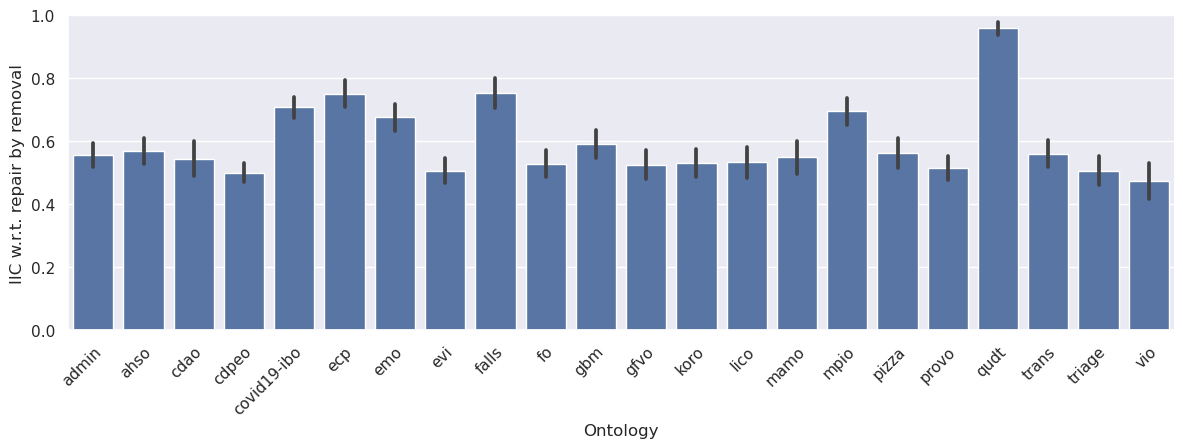
\includegraphics[width=\textwidth]{figures/iic-remove-ontology-bar.png}
  \caption{Mean IIC with respect to repair via removal per ontology. The error bars show the 95\% confidence interval.}
  \label{fig:results-remove}
\end{figure}

\begin{figure}
  \centering
  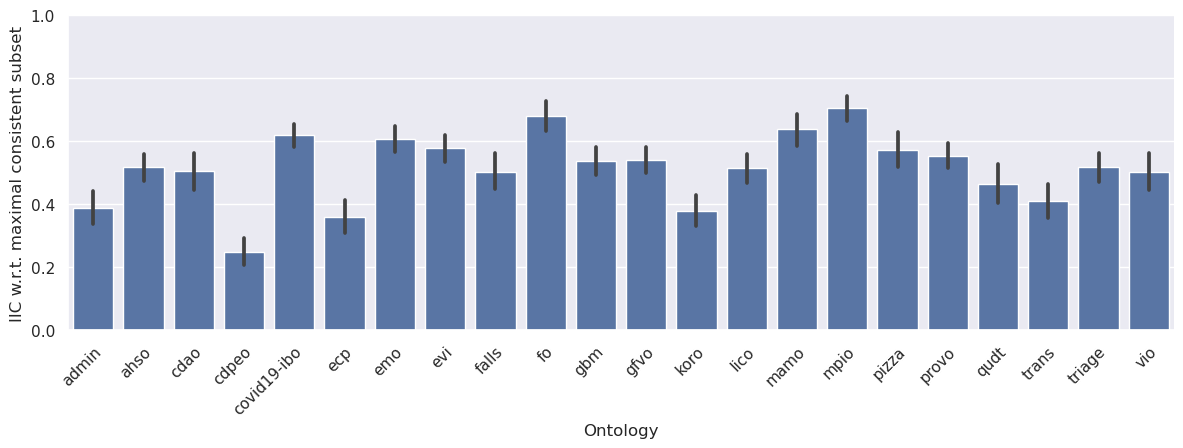
\includegraphics[width=\textwidth]{figures/iic-mcs-ontology-bar.png}
  \caption{Mean IIC with respect to a random maximal consistent subset per ontology. The error bars show the 95\% confidence interval.}
  \label{fig:results-mcs}
\end{figure}

The results of the evaluation suggest that the repair by weakening is on average about as good or better than the repair by removal of axioms. While this supports the conclusion in \cite{troquard2018repairing} that weakening is able to retain more information than removal, the observed advantage was worse than what has been observed in \cite{troquard2018repairing}. In contrast, it can be seen that the repair using weakening is not in general better than choosing a random maximal consistent subset. There are ontologies for which the repairs by weakening are on average significantly worse when comparing using IIC. This is however a somewhat unequal comparison. An alternative repair algorithm could start with a maximal consistent subset and use weakening to add in more information from the remaining axioms. Still, this result suggests that the heuristic used for selecting bad axioms is not reliable for preserving information, at least with respect to the chosen measure.

\section{Conclusions and Outlook}

% what have we done?
% better measures for comparing ontologies
% better heuristics to steer the algorithm
% complex roles in up and down covers
% more permissive refinement of role inclusions
We have proposed refinement operators and an axiom weakening operator for all aspects of \SROIQ and shown that for repairs of inconsistent ontologies weakening can, in some cases, significantly outperform removal. Further additions to the refinement operators may be studied, e.g., using non-simple roles in the upward and downward covers in certain contexts. Relaxing the allowed weakening for RIAs may also be considered, and to cover also extensions to regularity conditions such as those studied in \cite{DBLP:conf/cade/Kazakov10}. We have also seen that the repair algorithm likely needs better heuristics to steer the selection of bad and weakened axioms in order to result in better repairs. Future work could further focus on finding robust measures for comparing the quality of repairs.

%%
%% Define the bibliography file to be used
\bibliography{biblio}

%%
%% If your work has an appendix, this is the place to put it.
\cleardoublepage

\appendix

\section{Proofs of Results}
\paragraph{Lemma~\ref{lem:weaker}.}
%\begin{lemma}\ref{lem:weaker}
{\it   For every \SROIQ\  axiom $\phi$, if $\phi' \in g_{\Omcref,\Omcfull}(\phi)$, then $\phi \models_\Omcref \phi'$
}
%\end{lemma}

\begin{proof} We will handle each type of axiom separately.
  \begin{itemize}
    \item If $\phi = C \sqsubseteq D$, suppose $\phi' = C' \sqsubseteq D'$. From \Cref{lem:basic}.\ref{lem:generalisation} we know that $C' \sqsubseteq_\Omcref C$ and $D \sqsubseteq_\Omcref D'$. By transitivity of subsumption, we conclude that $C \sqsubseteq D \models_\Omcref C' \sqsubseteq D'$.
    \item If $\phi = C(a)$, suppose $\phi' = C'(a)$. From \Cref{lem:basic}.\ref{lem:generalisation} we know that $C \sqsubseteq_\Omcref C'$. Given any model $I$ of $\Omcref \cup \{ \phi \}$, $a^I \in C^I$. Since $C^I \subseteq C'^I$ in every model of $\Omcref$, $a^I \in C'^I$. We conclude that $C(a) \models_\Omcref C'(a)$.
    \item If $\phi = R(a, b)$, suppose $\phi' = R'(a, b)$. From \Cref{lem:basic}.\ref{lem:generalisation} we know that $R \sqsubseteq_\Omcref R'$. Given any model $I$ of $\Omcref \cup \{ \phi \}$, $\langle a^I, b^I \rangle \in R^I$. Since $R^I \subseteq R'^I$ in every model of $\Omcref$, $\langle a^I, b^I \rangle \in R'^I$. We conclude that $R(a, b) \models_\Omcref R'(a, b)$.
    \item If $\phi = \lnot R(a, b)$, suppose $\phi' = R'(a, b)$. From \Cref{lem:basic}.\ref{lem:generalisation} we know that $R' \sqsubseteq_\Omcref R$. Given any model $I$ of $\Omcref \cup \{ \phi \}$, $\langle a^I, b^I \rangle \not\in R^I$. Since $R'^I \subseteq R^I$ in every model of $\Omcref$, $\langle a^I, b^I \rangle \not\in R'^I$. We conclude that $\lnot R(a, b) \models_\Omcref \lnot R'(a, b)$.
    \item If $\phi = \disjoint(R, S)$, suppose $\phi' = \disjoint(R', S')$. From \Cref{lem:basic}.\ref{lem:generalisation} we know that $R' \sqsubseteq_\Omcref R$ and $S' \sqsubseteq_\Omcref S$. Given any model $I$ of $\Omcref \cup \{ \phi \}$, $R^I \cap S^I = \emptyset$. Since $R'^I \subseteq R^I$ and $S'^I \subseteq S^I$ in every model of $\Omcref$, $R'^I \cap S'^I = \emptyset$. We conclude that $\disjoint(R, S) \models_\Omcref \disjoint(R', S')$.
    \item If $\phi = S_1 \circ \cdots \circ S_n \sqsubseteq R$, suppose $\phi' = S_1' \circ \cdots \circ S_n' \sqsubseteq R'$. From \Cref{lem:basic}.\ref{lem:generalisation} we know that $R \sqsubseteq_\Omcref R'$ and $S_i' \sqsubseteq_\Omcref S_i$ for $i = 1, \dots, n$. Given any model $I$ of $\Omcref \cup \{ \phi \}$, $S_1^I \circ \cdots \circ S_n^I \subseteq R^I$. Since $R^I \subseteq R'^I$ and $S_i'^I \subseteq S_i^I$ for $i = 1, \dots, n$ in every model of $\Omcref$, $S_1'^I \circ \cdots \circ S_n'^I \subseteq R'^I$. We conclude that $S_1 \circ \cdots \circ S_n \sqsubseteq R \models_\Omcref S_1' \circ \cdots \circ S_n' \sqsubseteq R'$.
  \end{itemize}
\end{proof}

\paragraph{Lemma~\ref{lem:simple-roles}.}
%\begin{lemma} \label{lem:simple-roles}
{\it Let $\Omc$ be an ontology such that all simple roles of $\Omcfull$ are also simple in $\Omc$. For every axiom $\phi \in \Omc$ and role $R$, if $\phi' \in g_{\Omcref,\Omcfull}(\phi)$ and $R$ simple in $\Omc$, then $R$ is simple in $\Omc \cup \{ \phi' \}$.
}
%\end{lemma}

\begin{proof}(\emph{Sketch})
  For the addition to change the simplicity of any role, it must be that $\phi'$ is a RIA that has some role $R$ as the super role and is either complex, or for which the sub role is non-simple. Assume, by contradiction, that $R$ is a simple role in $\Omc$ and non-simple in $\Omc \cup \{ \phi' \}$. Since $R$ is simple in $\Omc$ it is not the universal, does not appear as the super role in any complex RIA of $\Omc$, and neither on the right-hand side of a simple RIA in $\Omc$ where the sub role is non-simple. If $\phi'$ is a complex RIA then, by definition of the weakening operator, $\phi$ must be a complex RIA and $R$ must also be the super role in $\phi$, making it non-simple in $\Omc$, which contradicts our assumption. Similarly, if $\phi'$ is a simple RIA with a non-simple role as the sub role, the sub role of $\phi$ must be equal to that of $\phi'$ because the refinement operators return only roles simple in $\Omcfull$, and those are also simple in $\Omc$. Further, since the super role of a RIA is only refined if the sub role is simple, $\phi' = \phi$, which means that $R$ is non-simple in $\Omc$, which contradicts the assumptions. It follows that such a role $R$ does not exist.
\end{proof}

\paragraph{Lemma \ref{lem:regularity}.}
%\begin{lemma} \label{lem:regularity}
{\it Let $\Omc$ be an ontology such that all simple roles of $\Omcfull$ are also simple in $\Omc$. For every axiom $\phi \in \Omc$, if $\phi' \in g_{\Omcref,\Omcfull}(\phi)$ and the RBox of $\Omc$ is regular, then the RBox of $\Omc \cup \{ \phi' \}$ is also regular.
  }
%\end{lemma}

\begin{proof}(\emph{Sketch}) \phantomsection\label{proof:regularity}
  Let us first argue that if there exists a preorder that satisfies the constraints necessary for checking regularity, then there exists $\preceq$ such that $S_1 \preceq S_2$, $S \preceq R$ and $R \not\preceq S$ for all simple roles $S, S_1, S_2$ and non-simple roles $R$. Firstly, $S_1 \not\preceq S_2$ and $S \not\preceq R$ cannot be required, because absence of a tuple is only required for complex RIAs, where the super role must not be a predecessor of the roles on the left-hand side. Since $S_1$ and $S$ are simple, they do not appear as the super role in a complex RIA. Similarly, $R \preceq S$ cannot be required. Since $S$ is simple and $R$ non-simple, it cannot be required directly through an axiom of the form $R \sqsubseteq S$. By induction, it cannot be required through transitivity, since $R \preceq T$ and $T \preceq S$ would have to be required. If $T$ is simple, $R \preceq T$ cannot be required, and if $T$ is non-simple, $T \preceq S$ cannot be required.

  Since $\Omc$ has a regular RBox, there exists such a $\preceq$ for $\Omc$. We will show that $\preceq$ is also a witness for regularity of $\Omc \cup \{ \phi' \}$. All RIA in $\Omc$ are of one of the allowed forms for $\preceq$. It is therefore sufficient to verify that $\phi'$ has one of the allowed forms.
  If $\phi' = \phi$ or $\phi'$ is not a RIA, it does not affect the regularity.
  Otherwise, if $\phi'$ is a simple RIA $S \sqsubseteq R$, then by definition of the weakening operator, $S$ is simple in $\Omcfull$, and therefore also in $\Omc$. Given that $S$ is simple, $S \preceq R$ holds for simple and non-simple $R$ by our choice of $\preceq$.
  If $\phi'$ is a complex RIA $S_1' \circ \cdots \circ S_n' \sqsubseteq R$, then $\phi$ is also a complex RIA $S_1 \circ \cdots \circ S_n \sqsubseteq R$ and $R$ is non-simple in $\Omc$. If $S_i \preceq R$ and $S_i \not\preceq R$, then so will $S_i' \preceq R$ and $R \not\preceq S_i'$, either because $S_i = S_i'$ or because $S_i'$ is simple and $R$ is non-simple. Since $\Omc$ has a regular RBox, the only case in which $R \preceq S_i$ is if $S_i = R$. In this case, $S_i' \preceq R$ and $R \not\preceq S_i'$ will still hold if $S_i \not= R$. If $S_i = R$, either $i = 0$ or $i = n$ which is allowed. The only delicate case is if $\phi = R \circ R \sqsubseteq R$, which will result in either $\phi' = S_1' \circ R \sqsubseteq R$ or $R \circ S_2' \sqsubseteq R$, both of which are valid.
\end{proof}

\paragraph{Theorem \ref{lem:global-constraints}.}
%\begin{theorem} \label{lem:global-constraints}
{\it
Given that $\Omcref$ and $\Omcfull$ are valid \SROIQ ontologies. For every axiom $\phi \in \Omcfull$, if $\phi' \in g_{\Omcref,\Omcfull}(\phi)$, then $\Omcfull \cup \{ \phi' \}$ is a valid \SROIQ ontology.
}
%\end{theorem}

\begin{proof}(\emph{Sketch})
  We have established already in \Cref{lem:regularity}, that the regularity of the RBox will be preserved.
  It is guaranteed by \Cref{lem:simple-roles} that all roles that were simple before addition, are still simple afterwards. Therefore, all usages of roles in axioms and concepts that were not touched by the refinement do not pose a problem. The condition static that the upcover and downcover of a role contain only roles that are simple in $\Omcfull$ (and therefore by \Cref{lem:simple-roles} also in $\Omcfull \cup \{ \phi' \}$) forces that every refinement of a role is simple. This restriction to simple roles guarantees that no non-simple role may be used in disjoint role axioms, or the scope of cardinality and self constraints.
\end{proof}

\end{document}

%%
%% End of file
